\documentclass[12pt,fleqn]{article}\usepackage{../../common}
\begin{document}
Ders 3

Örnek 

Bir önceki örneğin doğal bir uzantısı n-boyutlu reel kordinat uzayı
olabilir. Bu uzaydaki vektörler n-öğeli içinde n tane reel sayı olan bir
dizidirler, ve vektörler $x = (\xi_1, \xi_2,...,\xi_n)$
formundadırlar. Reel tek sayı $\xi_k$'ye vektörün $k$'inci elemanı adı
verilir. İki vektör, eğer tüm öğeleri birbirine eşit ise, eşittir. Sıfır
vektörü $\theta = (0,0,...,0)$ şeklinde tanımlıdır. 

$n$ boyutlu reel kordinat uzayı $\mathbb{R}^n$ olarak tanımlanır. Buna
tekabül eden n-öğeli kompleks sayıların uzayı $\mathbb{C}^n$'dir.

Bu noktada aslında boyut kavramını devreye sokmak için biraz erken. Daha
ileriki derslerde boyut kavramının detaylı tanımı yapılacak, ve bu
bahsettiğimiz uzayların hakikaten n-boyutlu olduğu ispatlanacak.

Örnek 

Sonsuz sayıda eleman, sonsuz öğeli dizi içeren vektörlerlerle ilginç bazı
uzaylar inşa edilebiliyor, ki bu uzayda tipik bir vektör vektörler
$x = (\xi_1, \xi_2,...,\xi_k,...)$ şeklinde oluyor. Diğer bir şekliyle
$x = \{\xi_k\} _{k=1}^{\infty}$.  Toplama ve çıkartma önceden olduğu gibi
teker teker, sırası birbirine uyan öğeler arasında yapılıyor. Reel
sayılardan oluşan her türlü sonsuz dizilerin listesi bir vektör uzayı
oluşturuyor. Bir dizi $\{\xi_k\}$'ye sınırlı (bounded) denir, eğer her $k$
için $|\xi_k| < M$ olacak şekilde bir $M$ sabiti var ise. Sonsuz ve sınırlı
(tanımını biraz önce yaptık) olan her dizi bir vektör uzayı oluşturur,
çünkü iki sınırlı dizinin birleşimi, ya da dizinin sayısal çarpımı yine bir
sınırlı dizi olacaktır.

Örnek 

İçinde sonlu / belirli (finite) miktarda sıfıra eşit olmayan öğe içeren tüm
dizilerin birleşimi bir vektör uzayıdır (her vektör -dizi- içinde farklı
miktarda sıfır olmayan öğe olabilir). Bu uzaya sonlu sayıda sıfırı olmayan
dizilerin uzayı ismi verilir. 

Örnek

Sonsuz tane reel sayıdan oluşan ve hepsi de sıfıra yaklaşan dizilerin
birleşimi bir vektör uzayıdır, çünkü bu tür sıfıra yaklaşan iki dizinin
toplamı da aynı şekilde sıfıra yaklaşır. Böyle bir dizinin skalar ile
'çarpımı, yani katı yine sıfıra yaklaşır. 

Örnek 

Reel çizgi üzerinde bir $[a,b]$ aralığı düşünün. Bu aralık üzerinde tanımlı
tüm sürekli fonksiyonlar bir vektör uzayı oluşturur. İki vektör $x,y$ daha
detaylı olarak $x(t),y(t)$ olarak kullanılıyor, ki $t \in [a,b]$. Eğer
$x = y$ ise $x(t) = y(t)$ demektir. $(x+y)(t) = x(t) + y(t)$ ve
$(\alpha x)(t) = \alpha x(t)$ kullanılır. Sıfır vektörü $\theta$ bu
aralıkta sürekli sıfır değerinde olan vektördür.  Bu uzaya [a,b] arasında
reel değerli sürekli fonksiyonlar uzayı denir.

$[a,b]$ aralığında tanımlı tüm sürekli fonksiyonların vektör uzayı
oluşturması mantıklı değil mi? Çünkü bir fonksiyon verilen bir değer için
bir başka değer üretmez mi? O zaman bu değerleri $[a,b]$ aralığına tekabül
eder şekilde yanyana düşünürsek, onlar da bir tür dizin
oluştururlar. Dizinin içeriği tabii ki fonksiyonun ne olduğuna göre
değişecektir, ama içerik sonuçta belli bir sayı dizisidir. Ve tüm bu farklı
dizinleri düşünürsek, onlar bir vektör uzayı oluşturabilirler. Ayrıca
\textbf{tüm} sürekli fonksiyonlardan bahsediliyor, bu neredeyse
\textbf{tüm} reel sayı dizileri demek gibi bir şey, çünkü $[a,b]$
aralığındaki her türlü fonksiyon uzaya dahil edilmiş. Her türlü kıvrılan,
bükülen, artan, azalan fonksiyonu düşünelim, bunların tamamı muhakkak bir
vektör uzayı tanımlayabilirler.

Şimdi birkaç vektör uzayını birleştirerek nasıl daha büyük bir tane
yaratabileceğimizi görelim. 

Tanım

$X,Y$'nin aynı skalar alanı üzerinden tanımlı iki vektör uzayı olduğunu
düşünelim. $X,Y$'nin kartezyen çarpımı, ki bu $X \times Y$ olarak
gösterilir, iki öğeli sıralanmış bir dizi oluşturacaktır, 
yani $(x,y)$, ki $ x \in X, y \in Y$. $X \times Y$ üzerinde toplama ve
skalar çarpım $(x_1,y_1) + (x_2,y_2) = (x_1+x_2, y_1+y_2)$ ve
$\alpha(x_1,y_1) = (\alpha x_1,\alpha y_1)$. 

Üstteki tanımın bir vektör uzayı olmanın gerekliliklerini yerine getirdiği
ortadadır. Hatta bu tanım kolaylıkla $n$ tane vektör uzayının kartezyen
çarpımına genişletilebilir, yani $X_1,X_2,..,X_n$. Bu çarpımı temsil etmek
için $X^n$ yazacağız. 

Alt Uzaylar (Subspaces), Lineer Kombinasyonlar, ve Lineer Çeşitler (Linear
Varieties)

Tanım 

$M$, $X$'in boş olmayan bir {\em alt uzayıdır} (subspace) eğer
$\alpha x + \beta y$ formundaki her vektör $M$ içinde ise, ve $x,y \in M$
olmak üzere.

Hiçbir alt uzayın boş olmadığını baştan kabul ettiğimize göre, içinde en az
bir $x$ olmalıdır. Tanım itibariyle ayrıca $0 x = \theta$'yi da
içermelidir, o zaman her alt uzay sıfır vektörünü de içerir. En basit alt
uzay içinde sadece $\theta$ olan alt uzaydır. Üç boyutlu uzayda orijinden
geçen bir düzlem bir alt uzay oluşturur, orijinden geçen bir çizgi aynı
şekilde bir alt uzay oluşturur.

$X$'in tamamı da $X$'in (yani kendisinin) bir alt uzayıdır. Tüm uzaya eşit
olmayan bir alt uzaya düzgün (proper) alt uzay denir.

Her alt uzay kendi öğelerinin toplamlarını, ve katlarını içerdiği için aynı
anda bir uzayı tanımlayan 7 gerekliliği (axiom) otomatik olarak yerine
getirmiş olur. Zaten alt uzay derken ``uzak'' kelimesini kullanabilmemizin
sebebi budur.

Diyelim ki $X$ uzayı $n$ öğeli dizinlerin (tuple) birleşimi. Bu dizinlerin
bir kopyasını düşünelim, tek farkla, 1. öğenin hep sıfır olsun. Bu bir alt
uzaydır. $1/2$ noktasında sıfır olan $[0,1]$ üzerinde tanımlı sürekli
fonksiyonlar, tüm sürekli fonksiyonların bir alt uzayıdır.

İki alt uzayın evliliği (union, $\cup$ ile gösterilen) bir alt uzay
olmayabilir. Bir düzlem üzerinde mesela, aynı yönde gitmeyen (noncolinear)
iki çizginin evliliği, bu iki ayrı çizginin rasgele toplamlarını içermediği
için alt uzay olma şartını yerine getirmez. Fakat ``kümelerin toplamı''
kavramından hareketle, iki alt uzay daha büyük bir alt uzay olarak özel bir
şekilde birleştirilebilir.

Tanım

Bir vektör uzayının $S,T$ adlı iki alt kümesinin toplamı $S+T$ olarak
gösterilir, ve her $s+t$ formundaki tüm vektörleri içerir, ki $s \in S,t
\in T$ olmak üzere. Dikkat, daha $S,T$'nin alt uzay olduğunu söylemiyoruz,
sadece küme diyoruz (şimdilik).

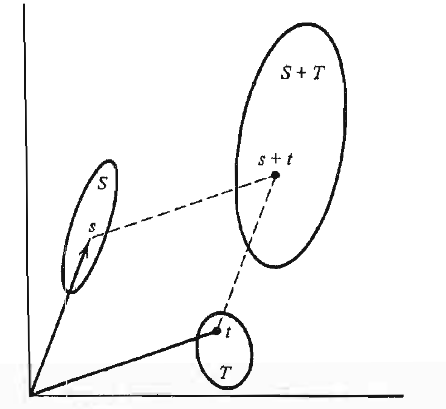
\includegraphics[height=5cm]{3_1.png}

Üstteki resim toplam kavramını iki boyutlu uzayda (ki bu bir vektör
uzayıdır) gösteriyor. Vektör uzayı, $S,T$ içindeki noktalara doğru işaret
eden orijinden çıkan iki vektörü görüyoruz. Toplam olarak, hakikaten
$S$'teki noktanın / vektörün mesela (3,1) olduğunu düşünsek, $T$'deki
noktanın / vektörün (1,3) olduğunu düşünsek, onların toplamı olarak
gösterilen nokta kabaca (4,4) gibi duruyor değil mi? Şekil bu kavramı
temsili olarak iyi göstermiş. Toplamın ayrıca daha büyük bir küme olduğuna
dikkat.

Teori 

Diyelim ki $M,N$ vektör uzayları $X$'in birer alt kümesi. O zaman bu kümelerin
toplamı $M + N$ aynı şekilde $X$'in bir alt uzayıdır. 

İspat 

$M+N$'nin $\theta$'yi içerdiği bariz. Devam edelim, $x,y \in S+T$ için
muhakkak 

$$ x = m_1 + n_1 $$

$$ y = m_2 + n_2 $$

var demektir, ki $m_1,m_2 \in M$, $n_1,n_2 \in N$. Bu küme toplamı
tanımından geliyor zaten. 

Şimdi $x,y$'yi ayrı ayrı rasgele sabitler $\alpha,\beta$ ile çarpalım. 

$$ \alpha x = \alpha m_1 + \alpha n_1 $$

$$ \beta y = \beta m_2 + \beta n_2 $$

Çarpımları toplayalım

$$ \alpha x + \beta y  = \alpha m_1 + \alpha n_1 + \beta m_2 + \beta n_2 $$

Eşitliğin sağını tekrar düzenleyelim

$$  \alpha x + \beta y  = (\alpha m_1 + \beta m_2) + (\alpha n_1  + \beta n_2 )$$

$\alpha x + \beta y $ ile $S+T$ içindeki $x+y$'nin herhangi bir şekildeki
katını almış oluyoruz. Ve geldiğimiz en son eşitlik gösteriyor 
ki $\alpha x + \beta y$ yine $M,N$ içindeki vektörlerin katları kullanılarak 
temsil edilebiliyor. Yani toplamdaki kat işlemini aynen alt kümelere
yansıtabiliyoruz / onların bazında yapabiliyoruz. O zaman alt kümeler alt
uzay olduğu için toplam da alt uzay demektir. İspat tamam.

İki boyutlu Öklit uzayında orijinden geçen ve aynı yönde olmayan iki çizginin
toplamı tüm uzaydır. 

Tanım

Vektör uzayındaki vektörler $x_1,x_2,..,x_n$'in lineer kombinasyonu
$\alpha_1 x_1 + \alpha_2 x_2 + ... + \alpha_n x_n$ olarak gösterilir. 

Daha önce vektör toplamı iki tane vektörün toplamı olarak
göstermiştik. Üstteki gibi $n$ tane toplam için (eski tanıma göre) toplam
ikişer ikişer yapılmalı tabii. Ve bunun doğal uzantısı olarak, alt
uzaydaki vektörlerin lineer kombinasyonu yine alt uzayda olacaktır. Ters
yönden bakarsak, bir vektör uzayının herhangi bir alt kümesinin lineer
kombinasyonlarını kullanarak bir alt uzayı yaratabiliriz. 

Tanım

Diyelim ki $S$ vektör uzayı $X$'in bir alt kümesi. {\em S tarafından
  üretilen alt uzay} yani $[S]$, $S$'teki elemanların lineer
kombinasyonu olan $X$'teki vektörlerden oluşur. 

\end{document}
